\section{Absorption on electrons}\label{sec:10.7}

A dark photon of \SI{10}{eV} that is absorbed in silicon deposits all of its energy, but at a momentum of only about \SI{10}{meV}, the momentum $\vect{p}_\phi = m_\phi\vect{v}$ it brings from the halo. A scattering particle that deposits the same \SI{10}{eV} needs at least $\omega/v_{\mathrm{max}} \approx \SI{4}{keV}$. Absorption therefore asks the crystal for its response at a single point, $\vect{q} \simeq 0$ and $\omega = m_\phi$, the point at which light probes it too (\cref{sec:1.4,sec:8.2-absorption}). The three standard bosons ask for three different functions at that point. The dark photon couples to the current of the electrons, and through its mixing with the photon of the medium it measures the loss function. The axion-like particle couples to the spin current of the electrons, which without spin--orbit coupling has the response of the current itself but no mixing, so the axion-like particle measures the optical conductivity. In a laboratory magnetic field it also couples through the photon, and then measures the loss function along the field. The scalar couples to the kinetic energy of the electrons, a response that no optical measurement provides.

\subsection{Dark-photon absorption and in-medium mixing}\label{sec:10.7-darkphoton}

\Cref{sec:8.4-mixing} found that a dark photon at rest is absorbed at the net rate $\varGamma_{\mathrm{net}} = \zeta^2m_\phi L(m_\phi)$, the loss function at $\vect{q} \to 0$, and that this rate is the familiar $\zeta_{\mathrm{eff}}^2\sigma_1$ with the in-medium mixing $\zeta_{\mathrm{eff}} = \zeta/\varepsilon$. A dark photon of the halo is not at rest, and it has three polarizations: two transverse to $\vect{p}_\phi$, which mix with the transverse photon of the medium, and one longitudinal, which mixes with the longitudinal one. Each mixes through its own self-energy, $\Pi_{\mathrm{T}} = \omega^2(1 - \varepsilon^{\mathrm{T}})$ and $\Pi_{\mathrm{L}} = (\omega^2 - p_\phi^2)(1 - \varepsilon)$ (\cref{sec:8.4-mixing}), both evaluated at $(\vect{p}_\phi, \omega)$ with $\omega^2 = m_\phi^2 + p_\phi^2$. The photon-reducible chain of \cref{app:D.25} applies to each polarization separately and replaces $\zeta^2$ by $\zeta^2m_\phi^4/|m_\phi^2 - \Pi_{\mathrm{T,L}}|^2$, and the net rate of each is $-1/\omega$ times the imaginary part of its proper self-energy times that factor~\cites[Eqs.~(2) and (18)]{an2015direct}[Eqs.~(38)--(40)]{mitridate2021dark}. For the longitudinal mode $m_\phi^2 - \Pi_{\mathrm{L}} = m_\phi^2\varepsilon$ exactly, as \cref{sec:8.4-mixing} found, and $\Imag\Pi_{\mathrm{L}} = -m_\phi^2\varepsilon_2$. For a transverse mode $m_\phi^2 - \Pi_{\mathrm{T}} = \omega^2\varepsilon^{\mathrm{T}} - p_\phi^2$ and $\Imag\Pi_{\mathrm{T}} = -\omega^2\varepsilon_2^{\mathrm{T}}$. With $\sigma_1 = \omega\varepsilon_2$,
\begin{equation}
  \varGamma_{\mathrm{L}} = \zeta^2\,\frac{m_\phi^2}{\omega^2}\,\frac{\sigma_1}{|\varepsilon|^2} , \qquad
  \varGamma_{\mathrm{T}} = \zeta^2\,\frac{m_\phi^4}{|\omega^2\varepsilon^{\mathrm{T}} - p_\phi^2|^2}\,\sigma_1^{\mathrm{T}} ,
  \label{eq:10.7-TL}
\end{equation}
with $\varepsilon$, $\varepsilon^{\mathrm{T}}$ and the conductivities at $(\vect{p}_\phi, \omega)$, and $\sigma_1^{\mathrm{T}} = \omega\varepsilon_2^{\mathrm{T}}$.

The transverse and longitudinal polarizations differ through the momentum against the size of the cell: $\varepsilon^{\mathrm{T}}$ and $\varepsilon$ both tend to the same $\varepsilon(\omega)$ as $\vect{p}_\phi \to 0$ (\cref{eq:4.4-ET}), and their dependence on $\vect{p}_\phi$ is of order $(p_\phi a)^2$, about $10^{-9}$ at \SI{10}{eV}. The polarizations also differ through $p_\phi^2/\omega^2 \simeq v^2 \approx 10^{-6}$. To first order in $p_\phi^2/\omega^2$, \cref{eq:10.7-TL} gives $\varGamma_{\mathrm{T}}/\varGamma_{\mathrm{L}} = 1 + v^2[2\Real(1/\varepsilon) - 1]$. The transverse factor $|\omega^2\varepsilon - p_\phi^2|$ could single out the transverse modes only where $|\varepsilon|$ itself falls to $v^2$. A fall of $|\varepsilon|$ to $v^2$ would need a medium whose $\varepsilon_2$ at the plasma frequency is below $10^{-6}$. Silicon has $\varepsilon_2 \approx 0.2$ there, and even a clean metal has orders of magnitude more than $10^{-6}$. Averaged over the three polarizations of an unpolarized field, and with $\omega_\phi \simeq m_\phi$, the rate per particle is therefore $\zeta^2m_\phi L(m_\phi)$ up to corrections of order $v^2$. In a cubic crystal $\varepsilon(\omega)$ is a scalar at $\vect{q} \to 0$, and the orientation of the polarization relative to the crystal does not matter either. Multiplication by the number density $\rho_\chi/m_\phi$ and division by $\rho_T$ (\cref{eq:8.2-abs}) give
\begin{keyresult}[Dark-photon absorption]
\begin{equation}
  \mathcal{R} = \frac{\rho_\chi}{\rho_T\,m_\phi}\,\zeta_{\mathrm{eff}}^2\,\sigma_1(m_\phi) = \frac{\rho_\chi}{\rho_T}\,\zeta^2\,L(m_\phi)\,\bigl[1 + O(v^2)\bigr] ,
  \label{eq:10.7-dp}
\end{equation}
with $\zeta_{\mathrm{eff}} = \zeta/\varepsilon(m_\phi)$ and $L = \varepsilon_2/|\varepsilon|^2$ at $\vect{q} \to 0$~\cites[Eq.~(7)]{hochberg2017absorption}[Eq.~(3)]{berlin2024absorption}. The mass of the dark photon cancels between the number density and the rate per particle; the rate per unit mass follows the loss function of the target.
\end{keyresult}
\noindent Where the target absorbs light strongly it also screens strongly, and the rate is small: at \SI{3}{eV} silicon has $|\varepsilon|^2 = 761$, and the dark photon is absorbed 761 times more weakly than the vacuum mixing $\zeta$ would suggest. Near the plasma frequency the reverse happens. At \SI{16.3}{eV} $\varepsilon_1$ crosses zero, and at the peak of the loss function, \SI{16.4}{eV} (\cref{sec:4.4}), $|\varepsilon|^2 = 0.049$ and the in-medium factor $1/|\varepsilon|^2 = 20$ enhances the rate; the dark photon converts into the plasmon. \Cref{fig:10-absorption}a shows the suppression and the enhancement, against the vacuum-mixing rate $\zeta^2\sigma_1$ that the medium would produce without the photon-reducible chain. Well above the valence plasma frequency, \SI{16.6}{eV} (\cref{sec:4.3}), $|1 - \varepsilon|$ is small, and it stays small through the $L$ and $K$ edges, since the core electrons add little to it, and the in-medium and vacuum-mixing rates meet. In silicon they agree to \SI{10}{\percent} for every mass above \SI{63}{eV}.

The nuclei add a current of their own, $\sum_\kappa Z_\kappa\vect{j}_\kappa$ in the row of \cref{sec:8.1-absorption}. In silicon it does not reach the electronic energies: the Born charges vanish, and the ionic part of $\varepsilon$ consists of weak two-phonon absorption far below the gap. In a polar crystal the same \cref{eq:10.7-dp} holds with the total dielectric function, and below the gap the rate peaks at the longitudinal optical phonon (\cref{sec:5.5,sec:8.4-mixing}).

The function $\sigma_1$ that enters \cref{eq:10.7-dp} is the optical conductivity of the material, the proper transverse current response of \cref{sec:4.4}, and it is measured. Ellipsometry, transmission and reflectance give $\varepsilon$ from the infrared to the vacuum ultraviolet, and x-ray absorption gives it above about \SI{30}{eV} through the atomic scattering factors $f_1 + \ii f_2$, with $\varepsilon_1 = 1 - (4\pi\alpha\nd_{\mathrm{at}}/m_e\omega^2)f_1$ and $\varepsilon_2 = (4\pi\alpha\nd_{\mathrm{at}}/m_e\omega^2)f_2$ for an atomic density $\nd_{\mathrm{at}}$. For silicon we use the optical constants of float-zone silicon at \SI{300}{K} from \SI{4}{meV} to \SI{40}{eV}~\cite{franta2017temperature}, the data of \cref{fig:4-siloss}, and the tables of Henke, Gullikson and Davis above~\cite{henke1993xray}; at \SI{40}{eV} the two data sets give $\varepsilon = 0.840 + 0.019\,\ii$ and $0.852 + 0.019\,\ii$. A calculation of $\sigma_1$ at $\vect{q} \to 0$ needs the electron--hole attraction near the gap, through the Bethe--Salpeter equation of \cref{sec:4.9}, and the local fields above it. For the dark photon and the axion-like particle, measured data are the better input wherever they exist at the right temperature, and \cref{sec:10.7-edge} examines that proviso.

\begin{figure}[tbp]
  \centering
  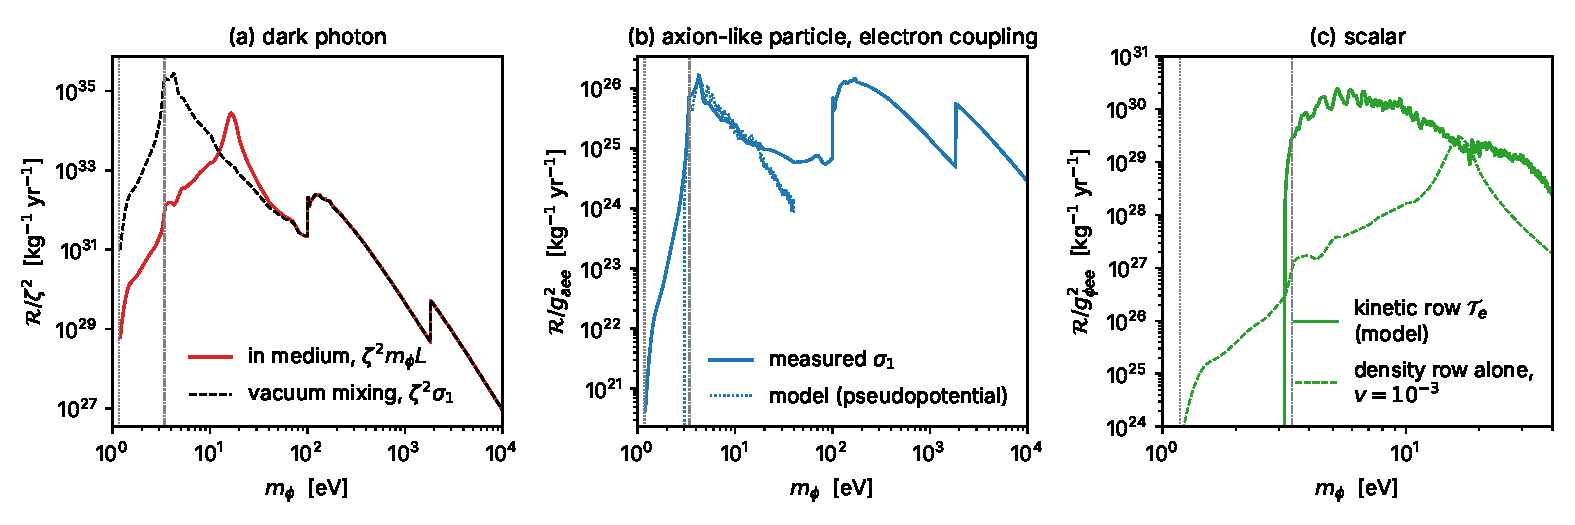
\includegraphics[width=\linewidth]{figures/ch10/fig10_6.pdf}
  \caption{Absorption rates of bosonic dark matter on the electrons of silicon, per kilogram-year and per unit squared coupling, against the boson mass $m_\phi$, with $\rho_\chi = \SI{0.3}{GeV.cm^{-3}}$ and $\rho_T = \SI{2.33}{g.cm^{-3}}$. Measured optical constants of float-zone silicon at \SI{300}{K}~\cite{franta2017temperature} below \SI{40}{eV}, and $\varepsilon$ from the atomic scattering factors of Ref.~\cite{henke1993xray} above, spliced at \SI{40}{eV}. The data are used without transfer to millikelvin temperatures and are wrong within a few tens of meV of the edge (\cref{sec:10.7-edge}). Dotted line: the excitonic edge of cold silicon, \SI{1.1728}{eV} with $\Eg(0) = \SI{1.1692}{eV}$; dash-dotted: the direct gap, \SI{3.4}{eV}. (a) Dark photon: in-medium rate $\zeta^2(\rho_\chi/\rho_T)L$, \cref{eq:10.7-dp} (red), and the vacuum-mixing rate $\zeta^2(\rho_\chi/\rho_T)\sigma_1/m_\phi$ (dashed). The same curve gives the axion-like particle in a field $\vect{B}_0$ with $\zeta \to g_{a\gamma\gamma}B_0/m_\phi$, \cref{eq:10.7-alpB}. (b) Axion-like particle with the electron coupling, \cref{eq:10.7-alp}, from the measured $\sigma_1$ (solid) and from the empirical-pseudopotential model of \cref{sec:4.6} (dotted; independent particles, no spin--orbit coupling, $16^3$ $\vect{k}$ points). (c) Scalar, \cref{eq:10.7-scalar}: kinetic-energy row in the same model, which has pseudo-wavefunctions without core oscillations and its own vertical gap of \SI{3.12}{eV} (solid; histogram of \SI{0.05}{eV} bins, smoothed over \SI{0.25}{eV}); and the screened density row alone at $|\vect{p}_\phi| = 10^{-3}m_\phi$ with the measured loss function (dashed). The model curves show the size and shape of the kinetic and spin responses, not predictions for silicon.}
  \label{fig:10-absorption}
\end{figure}

\begin{workedexample}{Dark-photon absorption at \SI{10}{eV}}\label{we:10-darkphoton}
At \SI{10}{eV} the measured dielectric function of silicon is $\varepsilon = -1.879 + 1.268\,\ii$: the frequency lies above the main interband peaks, where $\varepsilon_1$ has turned negative, and below the plasma frequency, where it turns positive again. Then $|\varepsilon|^2 = 5.139$, $L = \varepsilon_2/|\varepsilon|^2 = 0.2467$ and $\sigma_1 = \omega\varepsilon_2 = \SI{12.68}{eV}$. The in-medium mixing is $\zeta_{\mathrm{eff}}/\zeta = 1/|\varepsilon| = 0.441$, and the rate is suppressed by $1/|\varepsilon|^2 = 0.195$, a factor of 5.1. The photon self-energy is $\Pi_{\mathrm{em}} = m_\phi^2(1 - \varepsilon) = (288 - 127\,\ii)\,\mathrm{eV}^2$, larger than $m_\phi^2 = \SI{100}{eV^2}$.

With $\rho_\chi/m_\phi = \SI{3.0e7}{cm^{-3}}$, \cref{eq:10.7-dp} gives $\mathcal{R} = 1.52\times10^{33}\,\zeta^2$ per kilogram-year, against $7.82\times10^{33}\,\zeta^2$ with the vacuum mixing. Three events in a kilogram-year, the background-free reach, need $\zeta = 4.4\times10^{-17}$; the vacuum mixing would claim $2.0\times10^{-17}$, a reach better by $|\varepsilon| = 2.27$ than the true one. For a halo particle with $v = 10^{-3}$ the transverse and longitudinal rates differ by $v^2[2\Real(1/\varepsilon) - 1] = -1.7\times10^{-6}$, and each differs from \cref{eq:10.7-dp} at the level of $10^{-6}$.
\end{workedexample}

\subsection{Optical data near the silicon edge}\label{sec:10.7-edge}

Optical constants are measured at room temperature or at \SI{77}{K}, and a detector runs at \SI{10}{mK}. Above the direct gap of silicon, \SI{3.4}{eV}, the difference in temperature hardly matters: the transitions are vertical, the bands shift by tens of meV, and $\sigma_1$ changes little. Between the indirect gap and \SI{3.4}{eV} it matters a great deal. There every absorbed photon, and every absorbed dark-matter boson, needs a phonon to supply the crystal momentum $\vect{k}_{\mathrm{c}}$ of the conduction valley (\cref{sec:6.5}). The measured $\sigma_1$ in that window is the phonon-assisted $\omega\varepsilon_2^{\mathrm{PA}}$, second order in the electron--phonon vertex and first order in the phonon occupations, and it depends on temperature at the edge in two ways. At \SI{300}{K} the gap is \SI{1.12}{eV} instead of \SI{1.17}{eV}, and the transverse-acoustic phonon at $\vect{k}_{\mathrm{c}}$ has the occupation 0.97, so that a photon can be absorbed together with a phonon taken from the lattice, from $\Eg - \omega_{\mathrm{TA}}$ up. At \SI{10}{mK} no phonons are present to be absorbed, and the edge of cold silicon lies at $\Eg(0) + \omega_{\mathrm{TA}} - E_x^b = \SI{1.1728}{eV}$ with $\Eg(0) = \SI{1.1692}{eV}$, the excitonic threshold of phonon emission (\cref{sec:6.5}).

The consequence for a rate is direct. The \SI{300}{K} data give $\sigma_1 = 4.9\times10^{-4}$\,eV at \SI{1.15}{eV}, where a cold crystal absorbs nothing, and \cref{fig:10-absorption} inherits the warm edge. The \SI{77}{K} data are closer, but the occupation of the transverse-acoustic phonon is still 0.068 there, and the gap is \SI{1.165}{eV} against \SI{1.169}{eV} at millikelvin temperatures, from the measured temperature dependence of the gap~\cite{alex1996temperature} (\cref{sec:6.3}). Measured $\sigma_1$ near the edge must therefore be transferred to the temperature of the detector before it enters \cref{eq:10.7-dp} or the axion-like rate below. The transfer runs the phonon-assisted formula backward: each branch is separated into its absorption and emission parts, the absorption parts are removed, the emission parts are reweighted from $n_{\vect{Q}\nu} + 1$ to one, and the gap is shifted. Without data resolved by branch the separation is not unique. \Cref{sec:13.5} carries out the transfer and finds that the untransferred \SI{77}{K} data overestimate the millikelvin dark-photon rate of silicon by more than a factor of two within about \SI{20}{meV} of the edge.

\subsection{Axion-like-particle absorption}\label{sec:10.7-alp}

The axion-like particle couples to the electrons through \cref{eq:8.1-alp}, $(g_{aee}/m_e)[(\nabla\phi)\cdot\vect{s}_e + (\partial_t\phi)\mathcal{J}^{\alpha\alpha}_e]$ with the spin current traced over its two indices. For a particle of the halo the spin-density term is negligible. The coefficient of the spin-density term carries $|\vect{p}_\phi|$ instead of $m_\phi$. Without spin--orbit coupling the total spin also commutes with the Hamiltonian, so $\vect{s}_e(\vect{p}_\phi)$ connects different states only at first order in $\vect{p}_\phi$. The spin-density amplitude is then of order $p_\phi^2$, against $m_\phi$ times an electron velocity for the spin current. Only the row $\mathcal{J}_e \equiv \mathcal{J}^{\alpha\alpha}_e(0)$ is left, with $g^\phi_{\mathcal{J}} = g_{aee}m_\phi/m_e$ per unit amplitude, and \cref{eq:8.2-abs} gives $\varGamma = (g_{aee}^2m_\phi/2m_e^2)\,S_{\mathcal{J}\mathcal{J}}(0, m_\phi)$.

The spin current is related to the ordinary current by a spin trace. An electron--hole pair $(c\sigma', v\sigma)$ is created by $\mathcal{J}_e$ with the amplitude $\sum_\alpha v^\alpha_{cv}(S^\alpha)_{\sigma'\sigma}$, with $\vect{v}_{cv} = \langle c|\vect{p}/m_e|v\rangle$, and by the current along a unit vector $\hat{\vect{e}}$ with $\hat{\vect{e}}\cdot\vect{v}_{cv}\,\delta_{\sigma'\sigma}$. Summed over the spins, the spin-current amplitude gives $\sum_{\alpha\beta}v^\alpha_{cv}v^{\beta*}_{cv}\Tr(S^\alpha S^\beta) = |\vect{v}_{cv}|^2/2$, and the current amplitude gives $2|\hat{\vect{e}}\cdot\vect{v}_{cv}|^2$, which in a cubic crystal averages to $2|\vect{v}_{cv}|^2/3$. For independent electrons without spin--orbit coupling, therefore, $S_{\mathcal{J}\mathcal{J}} = \frac34 S_{jj}$, three Cartesian directions times the quarter that \cref{sec:10.5-triplet} found for every spin row. The transverse current response is the conductivity, $S_{jj}(0,\omega) = 2\omega\sigma_1/e^2$ (\cref{sec:4.4,sec:8.2-absorption}), and
\begin{keyresult}[Absorption of an axion-like particle through its electron coupling]
\begin{equation}
  \varGamma = \frac{3\,m_\phi^2}{4\,m_e^2}\,\frac{g_{aee}^2}{e^2}\,\sigma_1(m_\phi) , \qquad
  \mathcal{R} = \frac{\rho_\chi}{\rho_T\,m_\phi}\,\frac{3\,m_\phi^2\,g_{aee}^2}{4\,m_e^2\,e^2}\,\sigma_1(m_\phi) ,
  \label{eq:10.7-alp}
\end{equation}
for independent electrons without spin--orbit coupling~\cites[Eq.~(10)]{hochberg2017absorption}[Eq.~(47)]{mitridate2021dark}. There is no in-medium factor: the rate contains $\sigma_1$ in place of the loss function.
\end{keyresult}
\noindent The spin trace also explains the absence of mixing. A photon-reducible chain needs a proper correlation of $\mathcal{J}_e$ with the charge density, and a single spin operator traced over an unpolarized pair vanishes, $\Tr S^\alpha = 0$, so that $\tilde R_{\mathcal{J}Z} = 0$ (\cref{sec:8.4-mixing}). The parity of the particle says the same: a pseudoscalar cannot mix with the photon of a medium that has neither handedness nor magnetization~\cite[Sect.~III\,B, footnote~5]{mitridate2021dark}. Compared to the dark photon, then, the axion-like particle is not suppressed where the target absorbs light and not enhanced at the plasmon. At equal couplings the ratio of the axion-like rate to the dark-photon rate is $(3m_\phi^2/4m_e^2e^2)|\varepsilon|^2$, which at \SI{10}{eV} is $1.6\times10^{-8}$: the factor $m_\phi^2/m_e^2$ comes from a coupling to spin that a slow electron transmits only through its velocity. \Cref{fig:10-absorption}b shows the rate from the measured $\sigma_1$. The empirical-pseudopotential model of \cref{sec:4.6} gives 0.8 to 1.15 times the measured value between 4 and \SI{18}{eV}, and half of it at \SI{20}{eV}, far above the transitions to which its three form factors were fitted.

\Cref{eq:10.7-alp} uses the measured $\sigma_1$ for a response that differs from the one measured. The current creates electron--hole pairs in the spin singlet, and the spin current in the triplet. With the interaction switched on, the singlet pairs feel both kernels of the Bethe--Salpeter equation and the triplet pairs only the direct one, \cref{eq:10.5-triplet}. The excitonic attraction is common to the singlet and triplet pairs, and the measured edge carries it correctly. The local fields, however, which are the rest of the exchange kernel, act on the singlet pairs alone. In the model of \cref{sec:4.6} they lower the main $\varepsilon_2$ peak of silicon from 41 to 34 and move it up by \SI{60}{meV}. The measured $\sigma_1$ therefore understates the axion-like response near its peak by about a fifth, and by less where the local fields are weak. Spin--orbit coupling is the second caveat. It ties the spin to the orbital motion, the spin trace no longer factorizes, and the factor $\frac34$ acquires corrections set by the spin--orbit splitting over the transition energy, $\Delta_{\mathrm{SO}} = \SI{0.044}{eV}$ in silicon against several eV (\cref{sec:3.3}). In germanium, GaAs and heavier targets the current and spin-current responses must be computed separately.

The photon coupling, $g_{a\gamma\gamma}\phi\,\vect{E}\cdot\vect{B}$ of \cref{sec:1.4}, needs a field to act on. In a static laboratory field $\vect{B}_0$ it reads $g_{a\gamma\gamma}\phi\,\vect{E}\cdot\vect{B}_0 = -g_{a\gamma\gamma}\phi\,(\partial_t\vect{A})\cdot\vect{B}_0$ in the gauge without scalar potential, and after an integration by parts in time it is $\vect{J}_a\cdot\vect{A}$, with a source current along the field,
\begin{equation*}
  \vect{J}_a = g_{a\gamma\gamma}\,(\partial_t\phi)\,\vect{B}_0 ,
\end{equation*}
which oscillates at $m_\phi$ with the wavevector $\vect{p}_\phi$. The medium answers as it answers any current. For a sample much larger than the skin depth $(m_\phi\Imag\sqrt{\varepsilon})^{-1}$ its boundaries do not matter~\cite[footnote~1]{berlin2024absorption}, and at $\vect{p}_\phi \to 0$ the curl of the magnetic field drops out of the Amp\`ere--Maxwell law $\nabla\times\vect{B} = \vect{J} + \partial_t\vect{E}$ of \cref{sec:4.4}, with a relative error of order $p_\phi^2/\omega^2$. The induced current is $\vect{J}_{\mathrm{ind}} = \sigma_{\mathrm{cond}}\cdot\vect{E}$, with the conductivity tensor, so that $0 = \vect{J}_a + \sigma_{\mathrm{cond}}\cdot\vect{E} - \ii\omega\vect{E} = \vect{J}_a - \ii\omega\,\varepsilon\cdot\vect{E}$, by \cref{eq:4.4-sigma}. With the amplitude $\phi_0$ of $\phi = \Real(\phi_0\ee^{-\ii m_\phi t})$, $\vect{J}_a$ has the amplitude $-\ii m_\phi g_{a\gamma\gamma}\phi_0\vect{B}_0$, and the field is
\begin{equation*}
  \vect{E} = \frac{1}{\ii\omega}\,\varepsilon^{-1}\cdot\vect{J}_a = -g_{a\gamma\gamma}\,\phi_0\,\varepsilon^{-1}(m_\phi)\cdot\vect{B}_0 .
\end{equation*}
The power that this field dissipates per unit volume, averaged over a period, is $\frac12\Real(\vect{J}^*_{\mathrm{ind}}\cdot\vect{E}) = \frac{\omega}{2}\vect{E}^\dagger\cdot\varepsilon''\cdot\vect{E}$, with $\varepsilon'' = (\varepsilon - \varepsilon^\dagger)/2\ii$ the absorptive part of the tensor. Since $(\varepsilon^{-1})^\dagger(\varepsilon - \varepsilon^\dagger)\varepsilon^{-1} = (\varepsilon^{-1})^\dagger - \varepsilon^{-1}$, the power is $\frac{\omega}{2}g_{a\gamma\gamma}^2|\phi_0|^2\,\vect{B}_0\cdot\Imag[-\varepsilon^{-1}]\cdot\vect{B}_0$, where $\Imag[-\varepsilon^{-1}]$ denotes the absorptive part of $-\varepsilon^{-1}$. The number density of the field is its energy density $\frac12m_\phi^2|\phi_0|^2$ over $m_\phi$. Division of the power by the number density and by the energy $\omega$ of one quantum gives
\begin{keyresult}[Absorption of an axion-like particle in a static field]
\begin{equation}
  \varGamma = \frac{g_{a\gamma\gamma}^2B_0^2}{m_\phi}\;\hat{\vect{B}}_0\cdot\Imag\bigl[-\varepsilon^{-1}(m_\phi)\bigr]\cdot\hat{\vect{B}}_0 , \qquad
  \mathcal{R} = \frac{\rho_\chi}{\rho_T}\,\frac{g_{a\gamma\gamma}^2B_0^2}{m_\phi^2}\;\hat{\vect{B}}_0\cdot\Imag\bigl[-\varepsilon^{-1}\bigr]\cdot\hat{\vect{B}}_0 ,
  \label{eq:10.7-alpB}
\end{equation}
the inverse dielectric tensor projected on the direction of the field~\cite[Eqs.~(6) and (7)]{berlin2024absorption}. In a cubic crystal the projection is the loss function $L(m_\phi)$, and the rate equals the dark-photon rate with $\zeta = g_{a\gamma\gamma}B_0/m_\phi$.
\end{keyresult}
\noindent \Cref{fig:10-absorption}a gives the rate of the axion-like particle in a field for silicon with that substitution. A field of \SI{10}{T} is $B_0 = \SI{1953}{eV^2}$ in the units of \cref{app:A.2}, and with $g_{a\gamma\gamma} = \SI{e-10}{GeV^{-1}}$ the equivalent mixing at \SI{10}{eV} is $2.0\times10^{-17}$, or 0.58 events per kilogram-year in silicon. The field also acts on the target, through the Zeeman and orbital energies, but $\mu_{\mathrm{B}}B_0 = \SI{0.58}{meV}$ at \SI{10}{T} is negligible against electronic energies, and the derivation never used the symmetry of $\varepsilon$, only its absorptive part. The two couplings of the axion-like particle add without interference: the cross term needs a correlation of the spin current with the charge current, and this correlation vanishes without spin--orbit coupling for the same reason as $\tilde R_{\mathcal{J}Z}$.

In a crystal of lower symmetry the projection of the inverse is not the inverse of the projection. For a uniaxial crystal with the field at an angle $\theta$ to the optic axis, $\hat{\vect{B}}_0\cdot\varepsilon^{-1}\cdot\hat{\vect{B}}_0 = \cos^2\theta/\varepsilon_\parallel + \sin^2\theta/\varepsilon_\perp$, while the dielectric function along the field is $\varepsilon_{BB} = \cos^2\theta\,\varepsilon_\parallel + \sin^2\theta\,\varepsilon_\perp$, and
\begin{equation}
  \hat{\vect{B}}_0\cdot\varepsilon^{-1}\cdot\hat{\vect{B}}_0 - \frac{1}{\varepsilon_{BB}} = \frac{\cos^2\theta\,\sin^2\theta\,(\varepsilon_\parallel - \varepsilon_\perp)^2}{\varepsilon_\parallel\,\varepsilon_\perp\,\varepsilon_{BB}} .
  \label{eq:10.7-aniso}
\end{equation}
The difference is second order in the anisotropy and vanishes on the principal axes. Near a longitudinal resonance of one axis it is not small, because $1/\varepsilon_\parallel$ or $1/\varepsilon_\perp$ is large there while $\varepsilon_{BB}$ is not near zero. The isotropic formula with the dielectric function along the field then misses the resonance, and \cref{eq:10.7-alpB} keeps it.

\begin{limitbox}[Absorption with in-medium mixing][lim:10.7a]
Dark photon: $\mathcal{R} = (\rho_\chi/\rho_T m_\phi)\,\zeta_{\mathrm{eff}}^2\sigma_1(m_\phi)$, $\zeta_{\mathrm{eff}}^2 = \zeta^2m_\phi^4/|m_\phi^2 - \Pi_{\mathrm{em}}|^2$~\cite[Eqs.~(6) and (7)]{hochberg2017absorption}, which for $m_\phi^2 \gg |\Pi_{\mathrm{em}}|$ reduces to the vacuum mixing, $\varGamma = \zeta^2\sigma_1$~\cite[Eq.~(20)]{an2015direct}. Axion-like particle in a field: $\varGamma = (g_{a\gamma\gamma}B_0)^2\Imag[-1/\varepsilon(m_\phi)]/m_\phi$ for an isotropic target~\cite[Eq.~(7)]{berlin2024absorption}.
\par\smallskip
{\centering
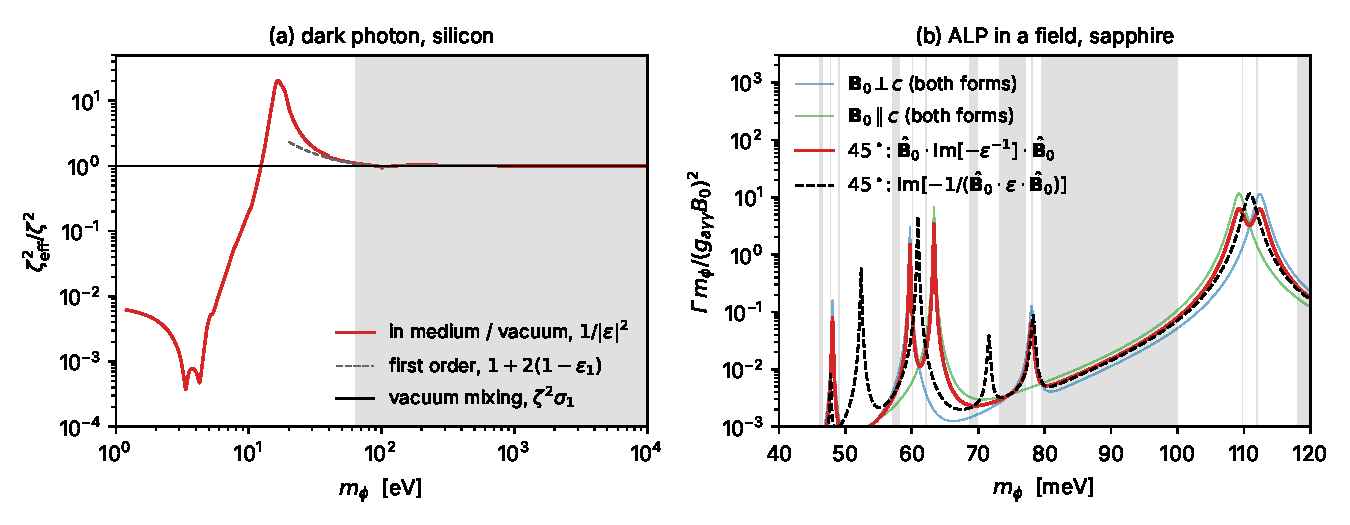
\includegraphics[width=\linewidth]{figures/ch10/limit10_7a.pdf}
\captionof{figure}{(a) Dark photon in silicon: the in-medium rate over the vacuum-mixing rate, $\zeta_{\mathrm{eff}}^2/\zeta^2 = 1/|\varepsilon(m_\phi)|^2$ (red), against the vacuum-mixing limit (black). Measured $\varepsilon$ at \SI{300}{K} below \SI{40}{eV}~\cite{franta2017temperature} and from atomic scattering factors above~\cite{henke1993xray}. Gray: masses where $1/|\varepsilon|^2$ is within \SI{10}{\percent} of one, all masses above \SI{63}{eV}. A halo momentum $|\vect{p}_\phi| = 10^{-3}m_\phi$ changes the transverse and longitudinal rates by $10^{-6}$, invisible here. (b) Axion-like particle in a field at \SI{45}{\degree} to the optic axis of sapphire: the rate of \cref{eq:10.7-alpB}, $\hat{\vect{B}}_0\cdot\Imag[-\varepsilon^{-1}]\cdot\hat{\vect{B}}_0$ (red), against the isotropic formula evaluated with the dielectric function along the field, $\Imag[-1/\varepsilon_{BB}]$ (dashed), and the two principal axes, where both forms agree (thin). Phonon dielectric functions of sapphire in the damped factorized form $\varepsilon = \varepsilon_\infty\prod_\nu(\omega_{\mathrm{L}\nu}^2 - \omega^2 - \ii\omega\gamma_{\mathrm{L}\nu})/(\omega_{\mathrm{T}\nu}^2 - \omega^2 - \ii\omega\gamma_{\mathrm{T}\nu})$ with $\varepsilon_\infty = 3.2$ and the frequencies and \SI{77}{K} widths of Ref.~\cite[Eq.~(37), Tables~I and II]{griffin2018directional} (ordinary ray, longitudinal 112.4, 78.0, 59.7 and \SI{48.1}{meV} with widths 1.98, 0.55, 0.17 and \SI{0.17}{meV}, transverse 78.6, 70.5, 54.4 and \SI{47.7}{meV} with widths 0.47, 0.40, 0.19 and \SI{0.17}{meV}; extraordinary ray, longitudinal 109.2 and \SI{63.3}{meV} with widths 1.98 and \SI{0.17}{meV}, transverse 72.2 and \SI{49.3}{meV} with widths 0.40 and \SI{0.19}{meV}), with the widths of the extraordinary ray borrowed from the ordinary modes. Gray: masses where the two forms agree within \SI{10}{\percent}. Silicon is cubic, and in silicon the two forms coincide.}\label{fig:10-abs-limit}
\par}
\smallskip
Below \SI{63}{eV} the medium changes the dark-photon rate of silicon by factors from $4\times10^{-4}$ to 20, and in an anisotropic crystal with the field off its principal axes the isotropic formula misses the longitudinal resonances of each axis by up to a factor of several hundred.
\end{limitbox}

\subsection{Scalar absorption and the kinetic-energy row}\label{sec:10.7-scalar}

A scalar coupled to $\bar\psi\psi$ acts on the target through \cref{eq:8.1-scalar}, $-g_{\phi ee}\phi\,[n_e(\vect{p}_\phi) - \mathcal{T}_e(\vect{p}_\phi)/m_e]$: on the number of electrons and, at next order in $1/m_e$, on their kinetic energy. For scattering the density row dominates. For absorption at $|\vect{p}_\phi| \approx 10^{-3}m_\phi$ the order is reversed: the density row connects different states only at first order in $\vect{p}_\phi$ and is suppressed by $v^2$ in the rate, while the kinetic row is not (\cref{sec:8.1-absorption}).

\Cref{sec:8.4-mixing} found that the scalar mixes with the photon through the proper correlations $\tilde R_{n_eZ}$ and $\tilde R_{\mathcal{T}_eZ}$ of its two rows with the charge. The correlation $\tilde R_{n_eZ}$ is the density response, of order $p_\phi^2$. For $\tilde R_{\mathcal{T}_eZ}$, expand in $\vect{p}_\phi$: $\tilde R_{\mathcal{T}_en_e}(\vect{p}_\phi,\omega) = \vect{p}_\phi\cdot\vect{F}(\omega) + O(p_\phi^2)$, where $\vect{F}$ is a vector built from the crystal alone. It must be invariant under every operation of the point group, and an invariant vector exists only in a polar group, one that leaves some direction fixed under every operation. Crystals with a polar group are pyroelectric: they carry a spontaneous electric polarization along that direction. Silicon ($O_h$), GaAs ($T_d$) and sapphire ($D_{3d}$) have no invariant vector, and in them $\tilde R_{\mathcal{T}_en_e} = O(p_\phi^2)$. The photon-reducible part, $\tilde R_{\mathcal{T}_eZ}\,v_{\mathrm{C}}(p_\phi)\,\varepsilon^{-1}\,\tilde R_{Z\mathcal{T}_e}$, is then of order $p_\phi^4\cdot e^2/p_\phi^2 = e^2p_\phi^2$ and vanishes with the density row. In a polar crystal, such as wurtzite GaN or ZnO, $\vect{F} \ne 0$ and the mixing survives at $\vect{p}_\phi \to 0$ as a term $(e^2/\omega^2)\,\hat{\vect{p}}_\phi\cdot\tilde R_{\mathcal{T}_e\vect{j}}\,\varepsilon^{-1}\,\tilde R_{\vect{j}\mathcal{T}_e}\cdot\hat{\vect{p}}_\phi$, with $n_e = \vect{p}_\phi\cdot\vect{j}_e/\omega$ on the energy shell (\cref{eq:4.3-continuity}). With only the kinetic row kept, and with $g^\phi_{\mathcal{T}_e} = g_{\phi ee}/m_e$ in \cref{eq:8.2-abs},
\begin{keyresult}[Scalar absorption]
\begin{equation}
  \varGamma = -\frac{g_{\phi ee}^2}{m_\phi\,m_e^2}\,\Imag R_{\mathcal{T}\mathcal{T}}(0, m_\phi) = \frac{g_{\phi ee}^2}{2\,m_\phi\,m_e^2}\,S_{\mathcal{T}\mathcal{T}}(0, m_\phi) ,
  \label{eq:10.7-scalar}
\end{equation}
with $R_{\mathcal{T}\mathcal{T}}$ the response of the kinetic-energy row $\mathcal{T}_e(0) = \sum_jp_j^2/2m_e$ at $T = 0$, for every crystal whose point group has no polar vector, up to corrections of order $v^2$ from the other rows~\cite[Eqs.~(55) and (56)]{mitridate2021dark}. The response is unscreened, and no optical measurement gives it.
\end{keyresult}
\noindent In the notation of Mitridate and collaborators the row is $\bar v^2 = \mathcal{T}_e/m_e$ and the coupling $d_{\phi ee}$, with $g_{\phi ee} = d_{\phi ee}\sqrt{4\pi}\,m_e/M_{\mathrm{Pl}}$ (\cref{sec:1.4}). For independent electrons the response is a joint density of states weighted by the kinetic matrix elements,
\begin{equation}
  S^0_{\mathcal{T}\mathcal{T}}(0,\omega) = \frac{4\pi}{\Vol}\sum_{cv\vect{k}}\bigl|\langle c\vect{k}|\mathcal{T}_e|v\vect{k}\rangle\bigr|^2\,\delta(\omega - \varepsilon_{c\vect{k}} + \varepsilon_{v\vect{k}}) ,
  \label{eq:10.7-S0}
\end{equation}
spin summed, with the one-electron element $\langle c|p^2/2m_e|v\rangle = \sum_m\vect{p}_{cm}\cdot\vect{p}_{mv}/2m_e$, a sum over all bands, the core included. Since $c$ and $v$ are eigenstates of $p^2/2m_e + V$ with different energies, the element is also $-\langle c|V|v\rangle$: the kinetic row measures the matrix elements of the crystal potential itself. Those are largest where the potential is deep, near the nuclei, and there a pseudo-wavefunction is smooth where the true state oscillates. The rate is therefore sensitive to the core region in a way that the conductivity is not, and a calculation needs the all-electron states or their reconstruction from a projector-augmented-wave basis.

The kinetic row also follows a different selection rule. It is even under inversion, while the momentum is odd. At $\mathrm{\Gamma}$ the top valence states of silicon and the lowest conduction states have opposite parity, and the opposite parity makes the direct transition at \SI{3.4}{eV} allowed for light. For the scalar the direct transition is forbidden: in the model of \cref{sec:4.6} the kinetic matrix element between them vanishes at $\mathrm{\Gamma}$ to machine precision, while the momentum element does not, and the scalar spectrum rises from the vertical gap more slowly than $\varepsilon_2$. Below the direct gap the scalar, like the dark photon, is absorbed only with a phonon, and its rate there needs the phonon-assisted kinetic row.

The kinetic row has a sum rule of its own. The first-moment identity \cref{eq:4.3-firstmoment} at $\vect{q} = 0$ gives $\int_0^\infty\dd\omega\,\omega\,S_{\mathcal{T}\mathcal{T}} = (\pi/\Vol)\langle[[\mathcal{T}_e, H], \mathcal{T}_e]\rangle$ at $T = 0$. Take electrons that move independently in a local one-body potential, $H = \sum_j[p_j^2/2m_e + V(\vect{r}_j)]$. With $\mathcal{T}_e = H - \sum_jV(\vect{r}_j)$ written in the outer commutator, the part with $H$ has zero expectation value in an eigenstate, and what remains is $-\langle[[\mathcal{T}_e, V], V]\rangle$. For one electron $[p^2, V] = -\ii(\vect{p}\cdot\nabla V + \nabla V\cdot\vect{p})$, and a second commutator with $V$ leaves $[[p^2, V], V] = -2|\nabla V|^2$. Per electron, then, $\frac12\langle[[\mathcal{T}_e, H], \mathcal{T}_e]\rangle = \langle|\nabla V|^2\rangle/2m_e$, and
\begin{equation}
  \int_0^\infty\dd\omega\;\omega\,S_{\mathcal{T}\mathcal{T}}(0,\omega) = \frac{\pi\,\nd_e}{m_e}\,\bigl\langle|\nabla V|^2\bigr\rangle ,
  \label{eq:10.7-sumrule}
\end{equation}
with the average taken per electron. Compared to the $f$-sum rule \cref{eq:4.3-fsum}, which has $\pi\nd_eq^2/m_e$, the squared momentum kick $q^2$ is replaced by the mean squared force on an electron. For the absorption rate the sum rule fixes $\int\dd m_\phi\,m_\phi^2\varGamma = \pi g_{\phi ee}^2\nd_e\langle|\nabla V|^2\rangle/2m_e^3$.

The conditions are restrictive: a potential that is local and one-body, and a mean squared force that is finite. A nonlocal pseudopotential keeps the identity in the form $-\langle[[\mathcal{T}_e,V_{\mathrm{NL}}],V_{\mathrm{NL}}]\rangle$, but the double commutator is then no longer $\langle|\nabla V|^2\rangle$, just as nonlocality changes the $f$-sum rule (\cref{eq:4.3-fsumNL}). The Coulomb repulsion between the electrons turns $\langle|\nabla V|^2\rangle$ into the mean squared total force on an electron, a two-body and three-body average. The decisive failure is the Coulomb potential of a nucleus, which makes the force diverge: $|\nabla V|^2 = Z^2\alpha^2/r^4$, and an $s$ state, with a finite density at the nucleus, gives $\int r^2\dd r/r^4 = \infty$. The valence states of silicon have s character inside the core, where they oscillate to stay orthogonal to the $1s$ and $2s$ states, so for the real crystal the right-hand side of \cref{eq:10.7-sumrule} is infinite. The spectrum of the kinetic row has a tail that decays too slowly for its first moment to converge, and \cref{eq:10.7-sumrule} cannot normalize it as the $f$-sum rule normalizes the density response. The sum rule does provide a check of a calculation within its own model, for a local and regular potential such as an empirical pseudopotential, or the valence block of a calculation whose potential is regular.

\begin{limitbox}[Scalar absorption through the kinetic-energy row][lim:10.7b]
$\varGamma = -(g_{\phi ee}^2/m_\phi m_e^2)\Imag R_{\mathcal{T}\mathcal{T}}(0, m_\phi)$, from the kinetic-energy term of the nonrelativistic scalar coupling~\cite[Eqs.~(18) and (56)]{mitridate2021dark}; its energy-weighted integral is \cref{eq:10.7-sumrule} for a local, regular one-body potential.
\par\smallskip
{\centering
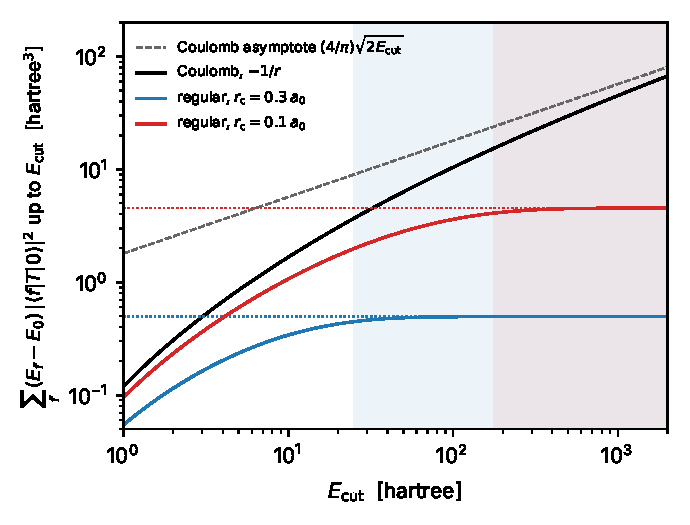
\includegraphics[width=0.66\linewidth]{figures/ch10/limit10_7b.pdf}
\captionof{figure}{Energy-weighted spectrum of the kinetic row, $\sum_f(E_f - E_0)|\langle f|p^2/2m_e|0\rangle|^2$ over final states up to an excitation energy $E_{\mathrm{cut}}$, for one electron in its ground state (atomic units), against $E_{\mathrm{cut}}$. Black: Coulomb potential $-1/r$, hydrogen; dashed, its asymptote $(4/\pi)\sqrt{2E_{\mathrm{cut}}}$, from the plane-wave limit of the continuum states. Blue and red: the regular potentials $-1/(r^2 + r_{\mathrm{c}}^2)^{1/2}$ with $r_{\mathrm{c}} = 0.3$ and $0.1\,a_0$; dotted, their sum rules $\langle|\nabla V|^2\rangle/2$, \cref{eq:10.7-sumrule}. Shaded: $E_{\mathrm{cut}}$ above which each regular spectrum holds \SI{90}{\percent} of its sum rule, 25 and \SI{176}{hartree}. Only s states contribute, since the kinetic energy conserves angular momentum. Radial equation on a uniform grid of \SI{0.004}{a_0} in a box of \SI{30}{a_0}; on the full grid the spectral sum and the double commutator agree to six digits.}\label{fig:10-scalar-limit}
\par}
\smallskip
For the Coulomb potential of a nucleus the energy-weighted spectrum grows as $E_{\mathrm{cut}}^{1/2}$ without limit, so the sum rule exists only for regular potentials, and its value grows as the core radius shrinks.
\end{limitbox}

The empirical-pseudopotential model of \cref{sec:4.6} is local and regular, and it satisfies \cref{eq:10.7-sumrule} exactly within its basis of 113 plane waves. On a grid of $16^3$ $\vect{k}$ points the spectral first moment and the double commutator agree to six digits, at $\langle|\nabla V|^2\rangle/2m_e = 1.30\times10^3\,\mathrm{eV}^3$ per valence electron. Only \SI{2}{\percent} of the first moment lies below \SI{10}{eV} and \SI{41}{\percent} below \SI{40}{eV}. Even in a model with a regular potential, then, the sum rule is carried by transitions far above the masses that matter, and it constrains the low-energy spectrum only weakly. \Cref{fig:10-absorption}c shows the model's scalar rate in silicon: $9.8\times10^{29}\,g_{\phi ee}^2$ per kilogram-year at \SI{10}{eV}, four orders of magnitude above the axion-like rate at equal coupling. The comparison with the electron's momentum makes the ratio of the scalar to the axion-like rate plausible. The kinetic matrix elements are a few eV, so $\mathcal{T}_e/m_e \sim 10^{-5}$, while the axion-like amplitude carries $m_\phi/m_e$ times an electron velocity, $\sim 10^{-7}$. The absolute value of the model curve is not a prediction, for the reason given above, and an all-electron response fixes it.

The dashed curve of \cref{fig:10-absorption}c is the density row alone, screened with the measured loss function, $(g_{\phi ee}^2/2m_\phi)(2p_\phi^2/e^2)L$ at $|\vect{p}_\phi| = 10^{-3}m_\phi$. It is one of the terms of order $v^2$ in \cref{eq:10.7-scalar}. At \SI{5}{eV} it is $3\times10^{-3}$ of the model's kinetic rate and at \SI{10}{eV} $2\times10^{-2}$. Near the plasma frequency, however, the density row is enhanced by the same factor $1/|\varepsilon|^2$ that enhances the dark photon, and between 16 and \SI{18}{eV} it is as large as the model's kinetic rate. The all-electron calculation of Mitridate and collaborators finds the kinetic term dominant in silicon and germanium~\cite[Fig.~1 and Sect.~IV]{mitridate2021dark}; its kinetic matrix elements include the core oscillations that our model lacks. The other terms of order $v^2$, the cross term between the rows and the mixing through $\tilde R_{\mathcal{T}_eZ}$, are of the same size as the density row and have not been computed. Within a few eV of the plasma frequency the margin by which \cref{eq:10.7-scalar} holds is therefore open, and it is fixed by the same all-electron calculation, extended to order $p_\phi^2$.
